\documentclass[a4paper,12pt]{report}
%\documentclass[a4paper,10pt]{scrartcl}

\usepackage{gfsneohellenic}
\usepackage{xltxtra}
\usepackage{pdfpages}
\usepackage{xcolor}
\usepackage{fancybox, graphicx}
\usepackage{xgreek} % Greek hyphenation
\usepackage[scale=0.77]{geometry}
\usepackage{array}
\usepackage{multirow}

\setromanfont[Mapping=tex-text]{GFS Neohellenic}
\setsansfont[Mapping=tex-text]{GFS Neohellenic}
\setmonofont[Mapping=tex-text]{GFS Neohellenic}

\newcounter{nextyear}
\renewcommand{\thesection}{\Roman{section}}
\makeatletter
\renewcommand\part{%
  \if@openright
    \cleardoublepage
  \else
    \clearpage
  \fi
  \thispagestyle{empty}%   % Original »plain« replaced by »emptyx
  \if@twocolumn
    \onecolumn
    \@tempswatrue
  \else
    \@tempswafalse
  \fi
  \null\vfil
  \secdef\@part\@spart}
\makeatother

\title{
\vspace{-2.5cm}
\line(1,0){440}\\
\vspace{0.2cm}
ΔΣ Φοιτητικού Συλλόγου Πληροφορικής και Τηλεματικής\\
\vspace{0.3cm}
\line(1,0){440}\\
\vspace{0.2cm} 

\includegraphics[scale=0.22]{hua.png} \\
\line(1,0){400}\\
\vspace{0.5cm}

\includegraphics[scale=0.495]{xarokopeio.jpg}
\vspace{0.5cm}
\line(1,0){400}\\
}
\author{}
\date{
\vspace{0.2cm}
Έτος \the\year \space- \thenextyear
}

\begin{document}
\color{blue!20!black!95}
\setcounter{nextyear}{\year}
\addtocounter{nextyear}{1}
\centering
\doublebox{
\begin{minipage}{\hsize}\
\centering
\maketitle
\end{minipage}
}

\Roman{part}
\Roman{section}

\part{Το ΔΣ}
\pagenumbering{Roman}

\section[Μέλη ΔΣ]{Τα Μέλη του ΔΣ το έτος \the\year \space- \thenextyear \space είναι :}
\vspace{1cm}

\begin{Large}
\begin{center}
\begin{tabular}{|l|c|}
  \hline
  \multicolumn{1}{|c}{Θέση} & \multicolumn{1}{c|}{Ονοματεπώνυμο} \\
  \hline
  Πρόεδρος & Παναγιώτης Ευστρατιάδης \\ \hline
  Αντιπρόεδρος & Ανδρέας Γρίβας \\ \hline
  Ταμίας & Βασιλεία Παπαιωάννου \\ \hline
  Γενικός Γραμματέας & Χριστίνα Μπαμπασανίδη \\ \hline
  Ειδικός Γραμματέας & Ξενοφών Δρίτσουλας \\ \hline
  Μέλος Α' & - \\ \hline
  Μέλος Β' & - \\ \hline
\end{tabular}
\vspace{0.5cm}
\end{center}
\end{Large}

\begin{large}
\paragraph{}
Ως ΔΣ του Φοιτητικού Συλλόγου Πληροφορικής και Τηλεματικής δηλώνουμε υπεύθυνα πως έχουμε διαβάσει το καταστατικό λειτουργίας
του συλλόγου και δεσμευόμαστε να το τηρούμε και να το υπερασπίσουμε μέχρι το τέλος της θήτειας μας ή μέχρις ότου αλλάξει η διαδικασία ή το καταστατικό
μετά από απόφαση γενικής συνέλευσης.
\vspace{0.5cm}

\begin{center}
\begin{tabular}{>{\centering\arraybackslash}p{4.5cm} c >{\centering\arraybackslash}p{4.5cm} c >{\centering\arraybackslash}p{4.5cm}}
\centering
Ο Πρόεδρος && Ο Αντιπρόεδρος && Ο Ταμίας \\
&&&& \\
&&&& \\
\cline{1-1}  \cline{3-3}  \cline{5-5} \\
\end{tabular}
\end{center}

\vspace{0.5cm}

\begin{center}
\begin{tabular}{>{\centering\arraybackslash}p{4.5cm} c >{\centering\arraybackslash}p{4.5cm}}
\centering
Ο Γ.Γραμματέας && Ο Ε.Γραμματέας\\
&& \\
&& \\
\cline{1-1}  \cline{3-3}\\
\end{tabular}
\end{center}

\vspace{0.5cm}

\begin{center}
\begin{tabular}{>{\centering\arraybackslash}p{4.5cm} c >{\centering\arraybackslash}p{4.5cm}}
\centering
&Τα Μέλη&\\
&& \\
&& \\
\cline{1-1}  \cline{3-3}\\
\end{tabular}
\end{center}
\end{large}



\part{Τα Πρακτικά}
\pagenumbering{arabic}
\setcounter{section}{0}
\section{Συνεδρίαση ΔΣ}
\begin{Large}
\begin{tabular}{|l|>{\centering\arraybackslash}p{5.2cm}|}
\hline
Ημερομηνία & { \hspace{0.7cm}-\hspace{0.7cm}-\hspace{1.4cm}} \\ \hline
\end{tabular}
\end{Large}
\vspace{1cm}
\section{Συζητήθηκαν}
\begin{Large}
\begin{enumerate}
 \item \line(1,0){425} \\
 \line(1,0){425} \\
 \line(1,0){425} \\
 \item \line(1,0){425} \\
 \line(1,0){425} \\
 \line(1,0){425} \\
  \item \line(1,0){425} \\
 \line(1,0){425} \\
 \line(1,0){425} \\
  \item \line(1,0){425} \\
 \line(1,0){425} \\
 \line(1,0){425} \\
  \item \line(1,0){425} \\
 \line(1,0){425} \\
 \line(1,0){425} \\

\end{enumerate}
\begin{center}
\line(1,0){440} \\
\line(1,0){440} \\
\line(1,0){440} \\
\line(1,0){440} \\
\line(1,0){440} \\
\end{center}
\end{Large}
\newpage
\section{Προτάθηκαν για θέματα Γενικής Συνέλευσης}
\vspace{1cm}
\begin{Large}
\begin{enumerate}
 \item \line(1,0){425} \\
 \line(1,0){425} \\
 \item \line(1,0){425} \\
 \line(1,0){425} \\
  \item \line(1,0){425} \\
 \line(1,0){425} \\
  \item \line(1,0){425} \\
 \line(1,0){425} \\
  \item \line(1,0){425} \\
 \line(1,0){425} \\

\end{enumerate}
\begin{center}
\line(1,0){440} \\
\line(1,0){440} \\
\line(1,0){440} \\
\line(1,0){440} \\
\line(1,0){440} \\
\end{center}
\end{Large}


\vspace{1cm}
\begin{center}
\begin{tabular}{>{\centering\arraybackslash}p{4.5cm} c >{\centering\arraybackslash}p{4.5cm} c >{\centering\arraybackslash}p{4.5cm}}
\centering
Ο Πρόεδρος && Ο Αντιπρόεδρος && Ο Ταμίας \\
&&&& \\
&&&& \\
\cline{1-1}  \cline{3-3}  \cline{5-5} \\
\end{tabular}
\end{center}

\vspace{0.5cm}

\begin{center}
\begin{tabular}{>{\centering\arraybackslash}p{4.5cm} c >{\centering\arraybackslash}p{4.5cm}}
\centering
Ο Γ.Γραμματέας && Ο Ε.Γραμματέας\\
&& \\
&& \\
\cline{1-1}  \cline{3-3}\\
\end{tabular}
\end{center}

\vspace{0.5cm}
\newpage
\setcounter{section}{0}
\section{Συνεδρίαση ΔΣ}
\begin{Large}
\begin{tabular}{|l|>{\centering\arraybackslash}p{5.2cm}|}
\hline
Ημερομηνία & { \hspace{0.7cm}-\hspace{0.7cm}-\hspace{1.4cm}} \\ \hline
\end{tabular}
\end{Large}
\vspace{1cm}
\section{Συζητήθηκαν}
\begin{Large}
\begin{enumerate}
 \item \line(1,0){425} \\
 \line(1,0){425} \\
 \line(1,0){425} \\
 \item \line(1,0){425} \\
 \line(1,0){425} \\
 \line(1,0){425} \\
  \item \line(1,0){425} \\
 \line(1,0){425} \\
 \line(1,0){425} \\
  \item \line(1,0){425} \\
 \line(1,0){425} \\
 \line(1,0){425} \\
  \item \line(1,0){425} \\
 \line(1,0){425} \\
 \line(1,0){425} \\

\end{enumerate}
\begin{center}
\line(1,0){440} \\
\line(1,0){440} \\
\line(1,0){440} \\
\line(1,0){440} \\
\line(1,0){440} \\
\end{center}
\end{Large}
\newpage
\section{Προτάθηκαν για θέματα Γενικής Συνέλευσης}
\vspace{1cm}
\begin{Large}
\begin{enumerate}
 \item \line(1,0){425} \\
 \line(1,0){425} \\
 \item \line(1,0){425} \\
 \line(1,0){425} \\
  \item \line(1,0){425} \\
 \line(1,0){425} \\
  \item \line(1,0){425} \\
 \line(1,0){425} \\
  \item \line(1,0){425} \\
 \line(1,0){425} \\

\end{enumerate}
\begin{center}
\line(1,0){440} \\
\line(1,0){440} \\
\line(1,0){440} \\
\line(1,0){440} \\
\line(1,0){440} \\
\end{center}
\end{Large}


\vspace{1cm}
\begin{center}
\begin{tabular}{>{\centering\arraybackslash}p{4.5cm} c >{\centering\arraybackslash}p{4.5cm} c >{\centering\arraybackslash}p{4.5cm}}
\centering
Ο Πρόεδρος && Ο Αντιπρόεδρος && Ο Ταμίας \\
&&&& \\
&&&& \\
\cline{1-1}  \cline{3-3}  \cline{5-5} \\
\end{tabular}
\end{center}

\vspace{0.5cm}

\begin{center}
\begin{tabular}{>{\centering\arraybackslash}p{4.5cm} c >{\centering\arraybackslash}p{4.5cm}}
\centering
Ο Γ.Γραμματέας && Ο Ε.Γραμματέας\\
&& \\
&& \\
\cline{1-1}  \cline{3-3}\\
\end{tabular}
\end{center}

\vspace{0.5cm}
\newpage
\setcounter{section}{0}
\section{Συνεδρίαση ΔΣ}
\begin{Large}
\begin{tabular}{|l|>{\centering\arraybackslash}p{5.2cm}|}
\hline
Ημερομηνία & { \hspace{0.7cm}-\hspace{0.7cm}-\hspace{1.4cm}} \\ \hline
\end{tabular}
\end{Large}
\vspace{1cm}
\section{Συζητήθηκαν}
\begin{Large}
\begin{enumerate}
 \item \line(1,0){425} \\
 \line(1,0){425} \\
 \line(1,0){425} \\
 \item \line(1,0){425} \\
 \line(1,0){425} \\
 \line(1,0){425} \\
  \item \line(1,0){425} \\
 \line(1,0){425} \\
 \line(1,0){425} \\
  \item \line(1,0){425} \\
 \line(1,0){425} \\
 \line(1,0){425} \\
  \item \line(1,0){425} \\
 \line(1,0){425} \\
 \line(1,0){425} \\

\end{enumerate}
\begin{center}
\line(1,0){440} \\
\line(1,0){440} \\
\line(1,0){440} \\
\line(1,0){440} \\
\line(1,0){440} \\
\end{center}
\end{Large}
\newpage
\section{Προτάθηκαν για θέματα Γενικής Συνέλευσης}
\vspace{1cm}
\begin{Large}
\begin{enumerate}
 \item \line(1,0){425} \\
 \line(1,0){425} \\
 \item \line(1,0){425} \\
 \line(1,0){425} \\
  \item \line(1,0){425} \\
 \line(1,0){425} \\
  \item \line(1,0){425} \\
 \line(1,0){425} \\
  \item \line(1,0){425} \\
 \line(1,0){425} \\

\end{enumerate}
\begin{center}
\line(1,0){440} \\
\line(1,0){440} \\
\line(1,0){440} \\
\line(1,0){440} \\
\line(1,0){440} \\
\end{center}
\end{Large}


\vspace{1cm}
\begin{center}
\begin{tabular}{>{\centering\arraybackslash}p{4.5cm} c >{\centering\arraybackslash}p{4.5cm} c >{\centering\arraybackslash}p{4.5cm}}
\centering
Ο Πρόεδρος && Ο Αντιπρόεδρος && Ο Ταμίας \\
&&&& \\
&&&& \\
\cline{1-1}  \cline{3-3}  \cline{5-5} \\
\end{tabular}
\end{center}

\vspace{0.5cm}

\begin{center}
\begin{tabular}{>{\centering\arraybackslash}p{4.5cm} c >{\centering\arraybackslash}p{4.5cm}}
\centering
Ο Γ.Γραμματέας && Ο Ε.Γραμματέας\\
&& \\
&& \\
\cline{1-1}  \cline{3-3}\\
\end{tabular}
\end{center}

\vspace{0.5cm}
\newpage
\setcounter{section}{0}
\section{Συνεδρίαση ΔΣ}
\begin{Large}
\begin{tabular}{|l|>{\centering\arraybackslash}p{5.2cm}|}
\hline
Ημερομηνία & { \hspace{0.7cm}-\hspace{0.7cm}-\hspace{1.4cm}} \\ \hline
\end{tabular}
\end{Large}
\vspace{1cm}
\section{Συζητήθηκαν}
\begin{Large}
\begin{enumerate}
 \item \line(1,0){425} \\
 \line(1,0){425} \\
 \line(1,0){425} \\
 \item \line(1,0){425} \\
 \line(1,0){425} \\
 \line(1,0){425} \\
  \item \line(1,0){425} \\
 \line(1,0){425} \\
 \line(1,0){425} \\
  \item \line(1,0){425} \\
 \line(1,0){425} \\
 \line(1,0){425} \\
  \item \line(1,0){425} \\
 \line(1,0){425} \\
 \line(1,0){425} \\

\end{enumerate}
\begin{center}
\line(1,0){440} \\
\line(1,0){440} \\
\line(1,0){440} \\
\line(1,0){440} \\
\line(1,0){440} \\
\end{center}
\end{Large}
\newpage
\section{Προτάθηκαν για θέματα Γενικής Συνέλευσης}
\vspace{1cm}
\begin{Large}
\begin{enumerate}
 \item \line(1,0){425} \\
 \line(1,0){425} \\
 \item \line(1,0){425} \\
 \line(1,0){425} \\
  \item \line(1,0){425} \\
 \line(1,0){425} \\
  \item \line(1,0){425} \\
 \line(1,0){425} \\
  \item \line(1,0){425} \\
 \line(1,0){425} \\

\end{enumerate}
\begin{center}
\line(1,0){440} \\
\line(1,0){440} \\
\line(1,0){440} \\
\line(1,0){440} \\
\line(1,0){440} \\
\end{center}
\end{Large}


\vspace{1cm}
\begin{center}
\begin{tabular}{>{\centering\arraybackslash}p{4.5cm} c >{\centering\arraybackslash}p{4.5cm} c >{\centering\arraybackslash}p{4.5cm}}
\centering
Ο Πρόεδρος && Ο Αντιπρόεδρος && Ο Ταμίας \\
&&&& \\
&&&& \\
\cline{1-1}  \cline{3-3}  \cline{5-5} \\
\end{tabular}
\end{center}

\vspace{0.5cm}

\begin{center}
\begin{tabular}{>{\centering\arraybackslash}p{4.5cm} c >{\centering\arraybackslash}p{4.5cm}}
\centering
Ο Γ.Γραμματέας && Ο Ε.Γραμματέας\\
&& \\
&& \\
\cline{1-1}  \cline{3-3}\\
\end{tabular}
\end{center}

\vspace{0.5cm}
\newpage
\setcounter{section}{0}
\section{Συνεδρίαση ΔΣ}
\begin{Large}
\begin{tabular}{|l|>{\centering\arraybackslash}p{5.2cm}|}
\hline
Ημερομηνία & { \hspace{0.7cm}-\hspace{0.7cm}-\hspace{1.4cm}} \\ \hline
\end{tabular}
\end{Large}
\vspace{1cm}
\section{Συζητήθηκαν}
\begin{Large}
\begin{enumerate}
 \item \line(1,0){425} \\
 \line(1,0){425} \\
 \line(1,0){425} \\
 \item \line(1,0){425} \\
 \line(1,0){425} \\
 \line(1,0){425} \\
  \item \line(1,0){425} \\
 \line(1,0){425} \\
 \line(1,0){425} \\
  \item \line(1,0){425} \\
 \line(1,0){425} \\
 \line(1,0){425} \\
  \item \line(1,0){425} \\
 \line(1,0){425} \\
 \line(1,0){425} \\

\end{enumerate}
\begin{center}
\line(1,0){440} \\
\line(1,0){440} \\
\line(1,0){440} \\
\line(1,0){440} \\
\line(1,0){440} \\
\end{center}
\end{Large}
\newpage
\section{Προτάθηκαν για θέματα Γενικής Συνέλευσης}
\vspace{1cm}
\begin{Large}
\begin{enumerate}
 \item \line(1,0){425} \\
 \line(1,0){425} \\
 \item \line(1,0){425} \\
 \line(1,0){425} \\
  \item \line(1,0){425} \\
 \line(1,0){425} \\
  \item \line(1,0){425} \\
 \line(1,0){425} \\
  \item \line(1,0){425} \\
 \line(1,0){425} \\

\end{enumerate}
\begin{center}
\line(1,0){440} \\
\line(1,0){440} \\
\line(1,0){440} \\
\line(1,0){440} \\
\line(1,0){440} \\
\end{center}
\end{Large}


\vspace{1cm}
\begin{center}
\begin{tabular}{>{\centering\arraybackslash}p{4.5cm} c >{\centering\arraybackslash}p{4.5cm} c >{\centering\arraybackslash}p{4.5cm}}
\centering
Ο Πρόεδρος && Ο Αντιπρόεδρος && Ο Ταμίας \\
&&&& \\
&&&& \\
\cline{1-1}  \cline{3-3}  \cline{5-5} \\
\end{tabular}
\end{center}

\vspace{0.5cm}

\begin{center}
\begin{tabular}{>{\centering\arraybackslash}p{4.5cm} c >{\centering\arraybackslash}p{4.5cm}}
\centering
Ο Γ.Γραμματέας && Ο Ε.Γραμματέας\\
&& \\
&& \\
\cline{1-1}  \cline{3-3}\\
\end{tabular}
\end{center}

\vspace{0.5cm}
\newpage
\setcounter{section}{0}
\section{Συνεδρίαση ΔΣ}
\begin{Large}
\begin{tabular}{|l|>{\centering\arraybackslash}p{5.2cm}|}
\hline
Ημερομηνία & { \hspace{0.7cm}-\hspace{0.7cm}-\hspace{1.4cm}} \\ \hline
\end{tabular}
\end{Large}
\vspace{1cm}
\section{Συζητήθηκαν}
\begin{Large}
\begin{enumerate}
 \item \line(1,0){425} \\
 \line(1,0){425} \\
 \line(1,0){425} \\
 \item \line(1,0){425} \\
 \line(1,0){425} \\
 \line(1,0){425} \\
  \item \line(1,0){425} \\
 \line(1,0){425} \\
 \line(1,0){425} \\
  \item \line(1,0){425} \\
 \line(1,0){425} \\
 \line(1,0){425} \\
  \item \line(1,0){425} \\
 \line(1,0){425} \\
 \line(1,0){425} \\

\end{enumerate}
\begin{center}
\line(1,0){440} \\
\line(1,0){440} \\
\line(1,0){440} \\
\line(1,0){440} \\
\line(1,0){440} \\
\end{center}
\end{Large}
\newpage
\section{Προτάθηκαν για θέματα Γενικής Συνέλευσης}
\vspace{1cm}
\begin{Large}
\begin{enumerate}
 \item \line(1,0){425} \\
 \line(1,0){425} \\
 \item \line(1,0){425} \\
 \line(1,0){425} \\
  \item \line(1,0){425} \\
 \line(1,0){425} \\
  \item \line(1,0){425} \\
 \line(1,0){425} \\
  \item \line(1,0){425} \\
 \line(1,0){425} \\

\end{enumerate}
\begin{center}
\line(1,0){440} \\
\line(1,0){440} \\
\line(1,0){440} \\
\line(1,0){440} \\
\line(1,0){440} \\
\end{center}
\end{Large}


\vspace{1cm}
\begin{center}
\begin{tabular}{>{\centering\arraybackslash}p{4.5cm} c >{\centering\arraybackslash}p{4.5cm} c >{\centering\arraybackslash}p{4.5cm}}
\centering
Ο Πρόεδρος && Ο Αντιπρόεδρος && Ο Ταμίας \\
&&&& \\
&&&& \\
\cline{1-1}  \cline{3-3}  \cline{5-5} \\
\end{tabular}
\end{center}

\vspace{0.5cm}

\begin{center}
\begin{tabular}{>{\centering\arraybackslash}p{4.5cm} c >{\centering\arraybackslash}p{4.5cm}}
\centering
Ο Γ.Γραμματέας && Ο Ε.Γραμματέας\\
&& \\
&& \\
\cline{1-1}  \cline{3-3}\\
\end{tabular}
\end{center}

\vspace{0.5cm}
\newpage
\setcounter{section}{0}
\section{Συνεδρίαση ΔΣ}
\begin{Large}
\begin{tabular}{|l|>{\centering\arraybackslash}p{5.2cm}|}
\hline
Ημερομηνία & { \hspace{0.7cm}-\hspace{0.7cm}-\hspace{1.4cm}} \\ \hline
\end{tabular}
\end{Large}
\vspace{1cm}
\section{Συζητήθηκαν}
\begin{Large}
\begin{enumerate}
 \item \line(1,0){425} \\
 \line(1,0){425} \\
 \line(1,0){425} \\
 \item \line(1,0){425} \\
 \line(1,0){425} \\
 \line(1,0){425} \\
  \item \line(1,0){425} \\
 \line(1,0){425} \\
 \line(1,0){425} \\
  \item \line(1,0){425} \\
 \line(1,0){425} \\
 \line(1,0){425} \\
  \item \line(1,0){425} \\
 \line(1,0){425} \\
 \line(1,0){425} \\

\end{enumerate}
\begin{center}
\line(1,0){440} \\
\line(1,0){440} \\
\line(1,0){440} \\
\line(1,0){440} \\
\line(1,0){440} \\
\end{center}
\end{Large}
\newpage
\section{Προτάθηκαν για θέματα Γενικής Συνέλευσης}
\vspace{1cm}
\begin{Large}
\begin{enumerate}
 \item \line(1,0){425} \\
 \line(1,0){425} \\
 \item \line(1,0){425} \\
 \line(1,0){425} \\
  \item \line(1,0){425} \\
 \line(1,0){425} \\
  \item \line(1,0){425} \\
 \line(1,0){425} \\
  \item \line(1,0){425} \\
 \line(1,0){425} \\

\end{enumerate}
\begin{center}
\line(1,0){440} \\
\line(1,0){440} \\
\line(1,0){440} \\
\line(1,0){440} \\
\line(1,0){440} \\
\end{center}
\end{Large}


\vspace{1cm}
\begin{center}
\begin{tabular}{>{\centering\arraybackslash}p{4.5cm} c >{\centering\arraybackslash}p{4.5cm} c >{\centering\arraybackslash}p{4.5cm}}
\centering
Ο Πρόεδρος && Ο Αντιπρόεδρος && Ο Ταμίας \\
&&&& \\
&&&& \\
\cline{1-1}  \cline{3-3}  \cline{5-5} \\
\end{tabular}
\end{center}

\vspace{0.5cm}

\begin{center}
\begin{tabular}{>{\centering\arraybackslash}p{4.5cm} c >{\centering\arraybackslash}p{4.5cm}}
\centering
Ο Γ.Γραμματέας && Ο Ε.Γραμματέας\\
&& \\
&& \\
\cline{1-1}  \cline{3-3}\\
\end{tabular}
\end{center}

\vspace{0.5cm}
\newpage
\setcounter{section}{0}
\section{Συνεδρίαση ΔΣ}
\begin{Large}
\begin{tabular}{|l|>{\centering\arraybackslash}p{5.2cm}|}
\hline
Ημερομηνία & { \hspace{0.7cm}-\hspace{0.7cm}-\hspace{1.4cm}} \\ \hline
\end{tabular}
\end{Large}
\vspace{1cm}
\section{Συζητήθηκαν}
\begin{Large}
\begin{enumerate}
 \item \line(1,0){425} \\
 \line(1,0){425} \\
 \line(1,0){425} \\
 \item \line(1,0){425} \\
 \line(1,0){425} \\
 \line(1,0){425} \\
  \item \line(1,0){425} \\
 \line(1,0){425} \\
 \line(1,0){425} \\
  \item \line(1,0){425} \\
 \line(1,0){425} \\
 \line(1,0){425} \\
  \item \line(1,0){425} \\
 \line(1,0){425} \\
 \line(1,0){425} \\

\end{enumerate}
\begin{center}
\line(1,0){440} \\
\line(1,0){440} \\
\line(1,0){440} \\
\line(1,0){440} \\
\line(1,0){440} \\
\end{center}
\end{Large}
\newpage
\section{Προτάθηκαν για θέματα Γενικής Συνέλευσης}
\vspace{1cm}
\begin{Large}
\begin{enumerate}
 \item \line(1,0){425} \\
 \line(1,0){425} \\
 \item \line(1,0){425} \\
 \line(1,0){425} \\
  \item \line(1,0){425} \\
 \line(1,0){425} \\
  \item \line(1,0){425} \\
 \line(1,0){425} \\
  \item \line(1,0){425} \\
 \line(1,0){425} \\

\end{enumerate}
\begin{center}
\line(1,0){440} \\
\line(1,0){440} \\
\line(1,0){440} \\
\line(1,0){440} \\
\line(1,0){440} \\
\end{center}
\end{Large}


\vspace{1cm}
\begin{center}
\begin{tabular}{>{\centering\arraybackslash}p{4.5cm} c >{\centering\arraybackslash}p{4.5cm} c >{\centering\arraybackslash}p{4.5cm}}
\centering
Ο Πρόεδρος && Ο Αντιπρόεδρος && Ο Ταμίας \\
&&&& \\
&&&& \\
\cline{1-1}  \cline{3-3}  \cline{5-5} \\
\end{tabular}
\end{center}

\vspace{0.5cm}

\begin{center}
\begin{tabular}{>{\centering\arraybackslash}p{4.5cm} c >{\centering\arraybackslash}p{4.5cm}}
\centering
Ο Γ.Γραμματέας && Ο Ε.Γραμματέας\\
&& \\
&& \\
\cline{1-1}  \cline{3-3}\\
\end{tabular}
\end{center}

\vspace{0.5cm}
\newpage
\setcounter{section}{0}
\section{Συνεδρίαση ΔΣ}
\begin{Large}
\begin{tabular}{|l|>{\centering\arraybackslash}p{5.2cm}|}
\hline
Ημερομηνία & { \hspace{0.7cm}-\hspace{0.7cm}-\hspace{1.4cm}} \\ \hline
\end{tabular}
\end{Large}
\vspace{1cm}
\section{Συζητήθηκαν}
\begin{Large}
\begin{enumerate}
 \item \line(1,0){425} \\
 \line(1,0){425} \\
 \line(1,0){425} \\
 \item \line(1,0){425} \\
 \line(1,0){425} \\
 \line(1,0){425} \\
  \item \line(1,0){425} \\
 \line(1,0){425} \\
 \line(1,0){425} \\
  \item \line(1,0){425} \\
 \line(1,0){425} \\
 \line(1,0){425} \\
  \item \line(1,0){425} \\
 \line(1,0){425} \\
 \line(1,0){425} \\

\end{enumerate}
\begin{center}
\line(1,0){440} \\
\line(1,0){440} \\
\line(1,0){440} \\
\line(1,0){440} \\
\line(1,0){440} \\
\end{center}
\end{Large}
\newpage
\section{Προτάθηκαν για θέματα Γενικής Συνέλευσης}
\vspace{1cm}
\begin{Large}
\begin{enumerate}
 \item \line(1,0){425} \\
 \line(1,0){425} \\
 \item \line(1,0){425} \\
 \line(1,0){425} \\
  \item \line(1,0){425} \\
 \line(1,0){425} \\
  \item \line(1,0){425} \\
 \line(1,0){425} \\
  \item \line(1,0){425} \\
 \line(1,0){425} \\

\end{enumerate}
\begin{center}
\line(1,0){440} \\
\line(1,0){440} \\
\line(1,0){440} \\
\line(1,0){440} \\
\line(1,0){440} \\
\end{center}
\end{Large}


\vspace{1cm}
\begin{center}
\begin{tabular}{>{\centering\arraybackslash}p{4.5cm} c >{\centering\arraybackslash}p{4.5cm} c >{\centering\arraybackslash}p{4.5cm}}
\centering
Ο Πρόεδρος && Ο Αντιπρόεδρος && Ο Ταμίας \\
&&&& \\
&&&& \\
\cline{1-1}  \cline{3-3}  \cline{5-5} \\
\end{tabular}
\end{center}

\vspace{0.5cm}

\begin{center}
\begin{tabular}{>{\centering\arraybackslash}p{4.5cm} c >{\centering\arraybackslash}p{4.5cm}}
\centering
Ο Γ.Γραμματέας && Ο Ε.Γραμματέας\\
&& \\
&& \\
\cline{1-1}  \cline{3-3}\\
\end{tabular}
\end{center}

\vspace{0.5cm}
\newpage
\setcounter{section}{0}
\section{Συνεδρίαση ΔΣ}
\begin{Large}
\begin{tabular}{|l|>{\centering\arraybackslash}p{5.2cm}|}
\hline
Ημερομηνία & { \hspace{0.7cm}-\hspace{0.7cm}-\hspace{1.4cm}} \\ \hline
\end{tabular}
\end{Large}
\vspace{1cm}
\section{Συζητήθηκαν}
\begin{Large}
\begin{enumerate}
 \item \line(1,0){425} \\
 \line(1,0){425} \\
 \line(1,0){425} \\
 \item \line(1,0){425} \\
 \line(1,0){425} \\
 \line(1,0){425} \\
  \item \line(1,0){425} \\
 \line(1,0){425} \\
 \line(1,0){425} \\
  \item \line(1,0){425} \\
 \line(1,0){425} \\
 \line(1,0){425} \\
  \item \line(1,0){425} \\
 \line(1,0){425} \\
 \line(1,0){425} \\

\end{enumerate}
\begin{center}
\line(1,0){440} \\
\line(1,0){440} \\
\line(1,0){440} \\
\line(1,0){440} \\
\line(1,0){440} \\
\end{center}
\end{Large}
\newpage
\section{Προτάθηκαν για θέματα Γενικής Συνέλευσης}
\vspace{1cm}
\begin{Large}
\begin{enumerate}
 \item \line(1,0){425} \\
 \line(1,0){425} \\
 \item \line(1,0){425} \\
 \line(1,0){425} \\
  \item \line(1,0){425} \\
 \line(1,0){425} \\
  \item \line(1,0){425} \\
 \line(1,0){425} \\
  \item \line(1,0){425} \\
 \line(1,0){425} \\

\end{enumerate}
\begin{center}
\line(1,0){440} \\
\line(1,0){440} \\
\line(1,0){440} \\
\line(1,0){440} \\
\line(1,0){440} \\
\end{center}
\end{Large}


\vspace{1cm}
\begin{center}
\begin{tabular}{>{\centering\arraybackslash}p{4.5cm} c >{\centering\arraybackslash}p{4.5cm} c >{\centering\arraybackslash}p{4.5cm}}
\centering
Ο Πρόεδρος && Ο Αντιπρόεδρος && Ο Ταμίας \\
&&&& \\
&&&& \\
\cline{1-1}  \cline{3-3}  \cline{5-5} \\
\end{tabular}
\end{center}

\vspace{0.5cm}

\begin{center}
\begin{tabular}{>{\centering\arraybackslash}p{4.5cm} c >{\centering\arraybackslash}p{4.5cm}}
\centering
Ο Γ.Γραμματέας && Ο Ε.Γραμματέας\\
&& \\
&& \\
\cline{1-1}  \cline{3-3}\\
\end{tabular}
\end{center}

\vspace{0.5cm}
\newpage
\setcounter{section}{0}
\section{Συνεδρίαση ΔΣ}
\begin{Large}
\begin{tabular}{|l|>{\centering\arraybackslash}p{5.2cm}|}
\hline
Ημερομηνία & { \hspace{0.7cm}-\hspace{0.7cm}-\hspace{1.4cm}} \\ \hline
\end{tabular}
\end{Large}
\vspace{1cm}
\section{Συζητήθηκαν}
\begin{Large}
\begin{enumerate}
 \item \line(1,0){425} \\
 \line(1,0){425} \\
 \line(1,0){425} \\
 \item \line(1,0){425} \\
 \line(1,0){425} \\
 \line(1,0){425} \\
  \item \line(1,0){425} \\
 \line(1,0){425} \\
 \line(1,0){425} \\
  \item \line(1,0){425} \\
 \line(1,0){425} \\
 \line(1,0){425} \\
  \item \line(1,0){425} \\
 \line(1,0){425} \\
 \line(1,0){425} \\

\end{enumerate}
\begin{center}
\line(1,0){440} \\
\line(1,0){440} \\
\line(1,0){440} \\
\line(1,0){440} \\
\line(1,0){440} \\
\end{center}
\end{Large}
\newpage
\section{Προτάθηκαν για θέματα Γενικής Συνέλευσης}
\vspace{1cm}
\begin{Large}
\begin{enumerate}
 \item \line(1,0){425} \\
 \line(1,0){425} \\
 \item \line(1,0){425} \\
 \line(1,0){425} \\
  \item \line(1,0){425} \\
 \line(1,0){425} \\
  \item \line(1,0){425} \\
 \line(1,0){425} \\
  \item \line(1,0){425} \\
 \line(1,0){425} \\

\end{enumerate}
\begin{center}
\line(1,0){440} \\
\line(1,0){440} \\
\line(1,0){440} \\
\line(1,0){440} \\
\line(1,0){440} \\
\end{center}
\end{Large}


\vspace{1cm}
\begin{center}
\begin{tabular}{>{\centering\arraybackslash}p{4.5cm} c >{\centering\arraybackslash}p{4.5cm} c >{\centering\arraybackslash}p{4.5cm}}
\centering
Ο Πρόεδρος && Ο Αντιπρόεδρος && Ο Ταμίας \\
&&&& \\
&&&& \\
\cline{1-1}  \cline{3-3}  \cline{5-5} \\
\end{tabular}
\end{center}

\vspace{0.5cm}

\begin{center}
\begin{tabular}{>{\centering\arraybackslash}p{4.5cm} c >{\centering\arraybackslash}p{4.5cm}}
\centering
Ο Γ.Γραμματέας && Ο Ε.Γραμματέας\\
&& \\
&& \\
\cline{1-1}  \cline{3-3}\\
\end{tabular}
\end{center}

\vspace{0.5cm}
\newpage
\setcounter{section}{0}
\section{Συνεδρίαση ΔΣ}
\begin{Large}
\begin{tabular}{|l|>{\centering\arraybackslash}p{5.2cm}|}
\hline
Ημερομηνία & { \hspace{0.7cm}-\hspace{0.7cm}-\hspace{1.4cm}} \\ \hline
\end{tabular}
\end{Large}
\vspace{1cm}
\section{Συζητήθηκαν}
\begin{Large}
\begin{enumerate}
 \item \line(1,0){425} \\
 \line(1,0){425} \\
 \line(1,0){425} \\
 \item \line(1,0){425} \\
 \line(1,0){425} \\
 \line(1,0){425} \\
  \item \line(1,0){425} \\
 \line(1,0){425} \\
 \line(1,0){425} \\
  \item \line(1,0){425} \\
 \line(1,0){425} \\
 \line(1,0){425} \\
  \item \line(1,0){425} \\
 \line(1,0){425} \\
 \line(1,0){425} \\

\end{enumerate}
\begin{center}
\line(1,0){440} \\
\line(1,0){440} \\
\line(1,0){440} \\
\line(1,0){440} \\
\line(1,0){440} \\
\end{center}
\end{Large}
\newpage
\section{Προτάθηκαν για θέματα Γενικής Συνέλευσης}
\vspace{1cm}
\begin{Large}
\begin{enumerate}
 \item \line(1,0){425} \\
 \line(1,0){425} \\
 \item \line(1,0){425} \\
 \line(1,0){425} \\
  \item \line(1,0){425} \\
 \line(1,0){425} \\
  \item \line(1,0){425} \\
 \line(1,0){425} \\
  \item \line(1,0){425} \\
 \line(1,0){425} \\

\end{enumerate}
\begin{center}
\line(1,0){440} \\
\line(1,0){440} \\
\line(1,0){440} \\
\line(1,0){440} \\
\line(1,0){440} \\
\end{center}
\end{Large}


\vspace{1cm}
\begin{center}
\begin{tabular}{>{\centering\arraybackslash}p{4.5cm} c >{\centering\arraybackslash}p{4.5cm} c >{\centering\arraybackslash}p{4.5cm}}
\centering
Ο Πρόεδρος && Ο Αντιπρόεδρος && Ο Ταμίας \\
&&&& \\
&&&& \\
\cline{1-1}  \cline{3-3}  \cline{5-5} \\
\end{tabular}
\end{center}

\vspace{0.5cm}

\begin{center}
\begin{tabular}{>{\centering\arraybackslash}p{4.5cm} c >{\centering\arraybackslash}p{4.5cm}}
\centering
Ο Γ.Γραμματέας && Ο Ε.Γραμματέας\\
&& \\
&& \\
\cline{1-1}  \cline{3-3}\\
\end{tabular}
\end{center}

\vspace{0.5cm}
\newpage
\setcounter{section}{0}
\section{Συνεδρίαση ΔΣ}
\begin{Large}
\begin{tabular}{|l|>{\centering\arraybackslash}p{5.2cm}|}
\hline
Ημερομηνία & { \hspace{0.7cm}-\hspace{0.7cm}-\hspace{1.4cm}} \\ \hline
\end{tabular}
\end{Large}
\vspace{1cm}
\section{Συζητήθηκαν}
\begin{Large}
\begin{enumerate}
 \item \line(1,0){425} \\
 \line(1,0){425} \\
 \line(1,0){425} \\
 \item \line(1,0){425} \\
 \line(1,0){425} \\
 \line(1,0){425} \\
  \item \line(1,0){425} \\
 \line(1,0){425} \\
 \line(1,0){425} \\
  \item \line(1,0){425} \\
 \line(1,0){425} \\
 \line(1,0){425} \\
  \item \line(1,0){425} \\
 \line(1,0){425} \\
 \line(1,0){425} \\

\end{enumerate}
\begin{center}
\line(1,0){440} \\
\line(1,0){440} \\
\line(1,0){440} \\
\line(1,0){440} \\
\line(1,0){440} \\
\end{center}
\end{Large}
\newpage
\section{Προτάθηκαν για θέματα Γενικής Συνέλευσης}
\vspace{1cm}
\begin{Large}
\begin{enumerate}
 \item \line(1,0){425} \\
 \line(1,0){425} \\
 \item \line(1,0){425} \\
 \line(1,0){425} \\
  \item \line(1,0){425} \\
 \line(1,0){425} \\
  \item \line(1,0){425} \\
 \line(1,0){425} \\
  \item \line(1,0){425} \\
 \line(1,0){425} \\

\end{enumerate}
\begin{center}
\line(1,0){440} \\
\line(1,0){440} \\
\line(1,0){440} \\
\line(1,0){440} \\
\line(1,0){440} \\
\end{center}
\end{Large}


\vspace{1cm}
\begin{center}
\begin{tabular}{>{\centering\arraybackslash}p{4.5cm} c >{\centering\arraybackslash}p{4.5cm} c >{\centering\arraybackslash}p{4.5cm}}
\centering
Ο Πρόεδρος && Ο Αντιπρόεδρος && Ο Ταμίας \\
&&&& \\
&&&& \\
\cline{1-1}  \cline{3-3}  \cline{5-5} \\
\end{tabular}
\end{center}

\vspace{0.5cm}

\begin{center}
\begin{tabular}{>{\centering\arraybackslash}p{4.5cm} c >{\centering\arraybackslash}p{4.5cm}}
\centering
Ο Γ.Γραμματέας && Ο Ε.Γραμματέας\\
&& \\
&& \\
\cline{1-1}  \cline{3-3}\\
\end{tabular}
\end{center}

\vspace{0.5cm}
\newpage
\setcounter{section}{0}
\section{Συνεδρίαση ΔΣ}
\begin{Large}
\begin{tabular}{|l|>{\centering\arraybackslash}p{5.2cm}|}
\hline
Ημερομηνία & { \hspace{0.7cm}-\hspace{0.7cm}-\hspace{1.4cm}} \\ \hline
\end{tabular}
\end{Large}
\vspace{1cm}
\section{Συζητήθηκαν}
\begin{Large}
\begin{enumerate}
 \item \line(1,0){425} \\
 \line(1,0){425} \\
 \line(1,0){425} \\
 \item \line(1,0){425} \\
 \line(1,0){425} \\
 \line(1,0){425} \\
  \item \line(1,0){425} \\
 \line(1,0){425} \\
 \line(1,0){425} \\
  \item \line(1,0){425} \\
 \line(1,0){425} \\
 \line(1,0){425} \\
  \item \line(1,0){425} \\
 \line(1,0){425} \\
 \line(1,0){425} \\

\end{enumerate}
\begin{center}
\line(1,0){440} \\
\line(1,0){440} \\
\line(1,0){440} \\
\line(1,0){440} \\
\line(1,0){440} \\
\end{center}
\end{Large}
\newpage
\section{Προτάθηκαν για θέματα Γενικής Συνέλευσης}
\vspace{1cm}
\begin{Large}
\begin{enumerate}
 \item \line(1,0){425} \\
 \line(1,0){425} \\
 \item \line(1,0){425} \\
 \line(1,0){425} \\
  \item \line(1,0){425} \\
 \line(1,0){425} \\
  \item \line(1,0){425} \\
 \line(1,0){425} \\
  \item \line(1,0){425} \\
 \line(1,0){425} \\

\end{enumerate}
\begin{center}
\line(1,0){440} \\
\line(1,0){440} \\
\line(1,0){440} \\
\line(1,0){440} \\
\line(1,0){440} \\
\end{center}
\end{Large}


\vspace{1cm}
\begin{center}
\begin{tabular}{>{\centering\arraybackslash}p{4.5cm} c >{\centering\arraybackslash}p{4.5cm} c >{\centering\arraybackslash}p{4.5cm}}
\centering
Ο Πρόεδρος && Ο Αντιπρόεδρος && Ο Ταμίας \\
&&&& \\
&&&& \\
\cline{1-1}  \cline{3-3}  \cline{5-5} \\
\end{tabular}
\end{center}

\vspace{0.5cm}

\begin{center}
\begin{tabular}{>{\centering\arraybackslash}p{4.5cm} c >{\centering\arraybackslash}p{4.5cm}}
\centering
Ο Γ.Γραμματέας && Ο Ε.Γραμματέας\\
&& \\
&& \\
\cline{1-1}  \cline{3-3}\\
\end{tabular}
\end{center}

\vspace{0.5cm}
\newpage
\setcounter{section}{0}
\section{Συνεδρίαση ΔΣ}
\begin{Large}
\begin{tabular}{|l|>{\centering\arraybackslash}p{5.2cm}|}
\hline
Ημερομηνία & { \hspace{0.7cm}-\hspace{0.7cm}-\hspace{1.4cm}} \\ \hline
\end{tabular}
\end{Large}
\vspace{1cm}
\section{Συζητήθηκαν}
\begin{Large}
\begin{enumerate}
 \item \line(1,0){425} \\
 \line(1,0){425} \\
 \line(1,0){425} \\
 \item \line(1,0){425} \\
 \line(1,0){425} \\
 \line(1,0){425} \\
  \item \line(1,0){425} \\
 \line(1,0){425} \\
 \line(1,0){425} \\
  \item \line(1,0){425} \\
 \line(1,0){425} \\
 \line(1,0){425} \\
  \item \line(1,0){425} \\
 \line(1,0){425} \\
 \line(1,0){425} \\

\end{enumerate}
\begin{center}
\line(1,0){440} \\
\line(1,0){440} \\
\line(1,0){440} \\
\line(1,0){440} \\
\line(1,0){440} \\
\end{center}
\end{Large}
\newpage
\section{Προτάθηκαν για θέματα Γενικής Συνέλευσης}
\vspace{1cm}
\begin{Large}
\begin{enumerate}
 \item \line(1,0){425} \\
 \line(1,0){425} \\
 \item \line(1,0){425} \\
 \line(1,0){425} \\
  \item \line(1,0){425} \\
 \line(1,0){425} \\
  \item \line(1,0){425} \\
 \line(1,0){425} \\
  \item \line(1,0){425} \\
 \line(1,0){425} \\

\end{enumerate}
\begin{center}
\line(1,0){440} \\
\line(1,0){440} \\
\line(1,0){440} \\
\line(1,0){440} \\
\line(1,0){440} \\
\end{center}
\end{Large}


\vspace{1cm}
\begin{center}
\begin{tabular}{>{\centering\arraybackslash}p{4.5cm} c >{\centering\arraybackslash}p{4.5cm} c >{\centering\arraybackslash}p{4.5cm}}
\centering
Ο Πρόεδρος && Ο Αντιπρόεδρος && Ο Ταμίας \\
&&&& \\
&&&& \\
\cline{1-1}  \cline{3-3}  \cline{5-5} \\
\end{tabular}
\end{center}

\vspace{0.5cm}

\begin{center}
\begin{tabular}{>{\centering\arraybackslash}p{4.5cm} c >{\centering\arraybackslash}p{4.5cm}}
\centering
Ο Γ.Γραμματέας && Ο Ε.Γραμματέας\\
&& \\
&& \\
\cline{1-1}  \cline{3-3}\\
\end{tabular}
\end{center}

\vspace{0.5cm}
\newpage
\setcounter{section}{0}
\section{Συνεδρίαση ΔΣ}
\begin{Large}
\begin{tabular}{|l|>{\centering\arraybackslash}p{5.2cm}|}
\hline
Ημερομηνία & { \hspace{0.7cm}-\hspace{0.7cm}-\hspace{1.4cm}} \\ \hline
\end{tabular}
\end{Large}
\vspace{1cm}
\section{Συζητήθηκαν}
\begin{Large}
\begin{enumerate}
 \item \line(1,0){425} \\
 \line(1,0){425} \\
 \line(1,0){425} \\
 \item \line(1,0){425} \\
 \line(1,0){425} \\
 \line(1,0){425} \\
  \item \line(1,0){425} \\
 \line(1,0){425} \\
 \line(1,0){425} \\
  \item \line(1,0){425} \\
 \line(1,0){425} \\
 \line(1,0){425} \\
  \item \line(1,0){425} \\
 \line(1,0){425} \\
 \line(1,0){425} \\

\end{enumerate}
\begin{center}
\line(1,0){440} \\
\line(1,0){440} \\
\line(1,0){440} \\
\line(1,0){440} \\
\line(1,0){440} \\
\end{center}
\end{Large}
\newpage
\section{Προτάθηκαν για θέματα Γενικής Συνέλευσης}
\vspace{1cm}
\begin{Large}
\begin{enumerate}
 \item \line(1,0){425} \\
 \line(1,0){425} \\
 \item \line(1,0){425} \\
 \line(1,0){425} \\
  \item \line(1,0){425} \\
 \line(1,0){425} \\
  \item \line(1,0){425} \\
 \line(1,0){425} \\
  \item \line(1,0){425} \\
 \line(1,0){425} \\

\end{enumerate}
\begin{center}
\line(1,0){440} \\
\line(1,0){440} \\
\line(1,0){440} \\
\line(1,0){440} \\
\line(1,0){440} \\
\end{center}
\end{Large}


\vspace{1cm}
\begin{center}
\begin{tabular}{>{\centering\arraybackslash}p{4.5cm} c >{\centering\arraybackslash}p{4.5cm} c >{\centering\arraybackslash}p{4.5cm}}
\centering
Ο Πρόεδρος && Ο Αντιπρόεδρος && Ο Ταμίας \\
&&&& \\
&&&& \\
\cline{1-1}  \cline{3-3}  \cline{5-5} \\
\end{tabular}
\end{center}

\vspace{0.5cm}

\begin{center}
\begin{tabular}{>{\centering\arraybackslash}p{4.5cm} c >{\centering\arraybackslash}p{4.5cm}}
\centering
Ο Γ.Γραμματέας && Ο Ε.Γραμματέας\\
&& \\
&& \\
\cline{1-1}  \cline{3-3}\\
\end{tabular}
\end{center}

\vspace{0.5cm}
\newpage
\setcounter{section}{0}
\section{Συνεδρίαση ΔΣ}
\begin{Large}
\begin{tabular}{|l|>{\centering\arraybackslash}p{5.2cm}|}
\hline
Ημερομηνία & { \hspace{0.7cm}-\hspace{0.7cm}-\hspace{1.4cm}} \\ \hline
\end{tabular}
\end{Large}
\vspace{1cm}
\section{Συζητήθηκαν}
\begin{Large}
\begin{enumerate}
 \item \line(1,0){425} \\
 \line(1,0){425} \\
 \line(1,0){425} \\
 \item \line(1,0){425} \\
 \line(1,0){425} \\
 \line(1,0){425} \\
  \item \line(1,0){425} \\
 \line(1,0){425} \\
 \line(1,0){425} \\
  \item \line(1,0){425} \\
 \line(1,0){425} \\
 \line(1,0){425} \\
  \item \line(1,0){425} \\
 \line(1,0){425} \\
 \line(1,0){425} \\

\end{enumerate}
\begin{center}
\line(1,0){440} \\
\line(1,0){440} \\
\line(1,0){440} \\
\line(1,0){440} \\
\line(1,0){440} \\
\end{center}
\end{Large}
\newpage
\section{Προτάθηκαν για θέματα Γενικής Συνέλευσης}
\vspace{1cm}
\begin{Large}
\begin{enumerate}
 \item \line(1,0){425} \\
 \line(1,0){425} \\
 \item \line(1,0){425} \\
 \line(1,0){425} \\
  \item \line(1,0){425} \\
 \line(1,0){425} \\
  \item \line(1,0){425} \\
 \line(1,0){425} \\
  \item \line(1,0){425} \\
 \line(1,0){425} \\

\end{enumerate}
\begin{center}
\line(1,0){440} \\
\line(1,0){440} \\
\line(1,0){440} \\
\line(1,0){440} \\
\line(1,0){440} \\
\end{center}
\end{Large}


\vspace{1cm}
\begin{center}
\begin{tabular}{>{\centering\arraybackslash}p{4.5cm} c >{\centering\arraybackslash}p{4.5cm} c >{\centering\arraybackslash}p{4.5cm}}
\centering
Ο Πρόεδρος && Ο Αντιπρόεδρος && Ο Ταμίας \\
&&&& \\
&&&& \\
\cline{1-1}  \cline{3-3}  \cline{5-5} \\
\end{tabular}
\end{center}

\vspace{0.5cm}

\begin{center}
\begin{tabular}{>{\centering\arraybackslash}p{4.5cm} c >{\centering\arraybackslash}p{4.5cm}}
\centering
Ο Γ.Γραμματέας && Ο Ε.Γραμματέας\\
&& \\
&& \\
\cline{1-1}  \cline{3-3}\\
\end{tabular}
\end{center}

\vspace{0.5cm}
\newpage
\setcounter{section}{0}
\section{Συνεδρίαση ΔΣ}
\begin{Large}
\begin{tabular}{|l|>{\centering\arraybackslash}p{5.2cm}|}
\hline
Ημερομηνία & { \hspace{0.7cm}-\hspace{0.7cm}-\hspace{1.4cm}} \\ \hline
\end{tabular}
\end{Large}
\vspace{1cm}
\section{Συζητήθηκαν}
\begin{Large}
\begin{enumerate}
 \item \line(1,0){425} \\
 \line(1,0){425} \\
 \line(1,0){425} \\
 \item \line(1,0){425} \\
 \line(1,0){425} \\
 \line(1,0){425} \\
  \item \line(1,0){425} \\
 \line(1,0){425} \\
 \line(1,0){425} \\
  \item \line(1,0){425} \\
 \line(1,0){425} \\
 \line(1,0){425} \\
  \item \line(1,0){425} \\
 \line(1,0){425} \\
 \line(1,0){425} \\

\end{enumerate}
\begin{center}
\line(1,0){440} \\
\line(1,0){440} \\
\line(1,0){440} \\
\line(1,0){440} \\
\line(1,0){440} \\
\end{center}
\end{Large}
\newpage
\section{Προτάθηκαν για θέματα Γενικής Συνέλευσης}
\vspace{1cm}
\begin{Large}
\begin{enumerate}
 \item \line(1,0){425} \\
 \line(1,0){425} \\
 \item \line(1,0){425} \\
 \line(1,0){425} \\
  \item \line(1,0){425} \\
 \line(1,0){425} \\
  \item \line(1,0){425} \\
 \line(1,0){425} \\
  \item \line(1,0){425} \\
 \line(1,0){425} \\

\end{enumerate}
\begin{center}
\line(1,0){440} \\
\line(1,0){440} \\
\line(1,0){440} \\
\line(1,0){440} \\
\line(1,0){440} \\
\end{center}
\end{Large}


\vspace{1cm}
\begin{center}
\begin{tabular}{>{\centering\arraybackslash}p{4.5cm} c >{\centering\arraybackslash}p{4.5cm} c >{\centering\arraybackslash}p{4.5cm}}
\centering
Ο Πρόεδρος && Ο Αντιπρόεδρος && Ο Ταμίας \\
&&&& \\
&&&& \\
\cline{1-1}  \cline{3-3}  \cline{5-5} \\
\end{tabular}
\end{center}

\vspace{0.5cm}

\begin{center}
\begin{tabular}{>{\centering\arraybackslash}p{4.5cm} c >{\centering\arraybackslash}p{4.5cm}}
\centering
Ο Γ.Γραμματέας && Ο Ε.Γραμματέας\\
&& \\
&& \\
\cline{1-1}  \cline{3-3}\\
\end{tabular}
\end{center}

\vspace{0.5cm}
\newpage
\setcounter{section}{0}
\section{Συνεδρίαση ΔΣ}
\begin{Large}
\begin{tabular}{|l|>{\centering\arraybackslash}p{5.2cm}|}
\hline
Ημερομηνία & { \hspace{0.7cm}-\hspace{0.7cm}-\hspace{1.4cm}} \\ \hline
\end{tabular}
\end{Large}
\vspace{1cm}
\section{Συζητήθηκαν}
\begin{Large}
\begin{enumerate}
 \item \line(1,0){425} \\
 \line(1,0){425} \\
 \line(1,0){425} \\
 \item \line(1,0){425} \\
 \line(1,0){425} \\
 \line(1,0){425} \\
  \item \line(1,0){425} \\
 \line(1,0){425} \\
 \line(1,0){425} \\
  \item \line(1,0){425} \\
 \line(1,0){425} \\
 \line(1,0){425} \\
  \item \line(1,0){425} \\
 \line(1,0){425} \\
 \line(1,0){425} \\

\end{enumerate}
\begin{center}
\line(1,0){440} \\
\line(1,0){440} \\
\line(1,0){440} \\
\line(1,0){440} \\
\line(1,0){440} \\
\end{center}
\end{Large}
\newpage
\section{Προτάθηκαν για θέματα Γενικής Συνέλευσης}
\vspace{1cm}
\begin{Large}
\begin{enumerate}
 \item \line(1,0){425} \\
 \line(1,0){425} \\
 \item \line(1,0){425} \\
 \line(1,0){425} \\
  \item \line(1,0){425} \\
 \line(1,0){425} \\
  \item \line(1,0){425} \\
 \line(1,0){425} \\
  \item \line(1,0){425} \\
 \line(1,0){425} \\

\end{enumerate}
\begin{center}
\line(1,0){440} \\
\line(1,0){440} \\
\line(1,0){440} \\
\line(1,0){440} \\
\line(1,0){440} \\
\end{center}
\end{Large}


\vspace{1cm}
\begin{center}
\begin{tabular}{>{\centering\arraybackslash}p{4.5cm} c >{\centering\arraybackslash}p{4.5cm} c >{\centering\arraybackslash}p{4.5cm}}
\centering
Ο Πρόεδρος && Ο Αντιπρόεδρος && Ο Ταμίας \\
&&&& \\
&&&& \\
\cline{1-1}  \cline{3-3}  \cline{5-5} \\
\end{tabular}
\end{center}

\vspace{0.5cm}

\begin{center}
\begin{tabular}{>{\centering\arraybackslash}p{4.5cm} c >{\centering\arraybackslash}p{4.5cm}}
\centering
Ο Γ.Γραμματέας && Ο Ε.Γραμματέας\\
&& \\
&& \\
\cline{1-1}  \cline{3-3}\\
\end{tabular}
\end{center}

\vspace{0.5cm}
\newpage
\setcounter{section}{0}
\section{Συνεδρίαση ΔΣ}
\begin{Large}
\begin{tabular}{|l|>{\centering\arraybackslash}p{5.2cm}|}
\hline
Ημερομηνία & { \hspace{0.7cm}-\hspace{0.7cm}-\hspace{1.4cm}} \\ \hline
\end{tabular}
\end{Large}
\vspace{1cm}
\section{Συζητήθηκαν}
\begin{Large}
\begin{enumerate}
 \item \line(1,0){425} \\
 \line(1,0){425} \\
 \line(1,0){425} \\
 \item \line(1,0){425} \\
 \line(1,0){425} \\
 \line(1,0){425} \\
  \item \line(1,0){425} \\
 \line(1,0){425} \\
 \line(1,0){425} \\
  \item \line(1,0){425} \\
 \line(1,0){425} \\
 \line(1,0){425} \\
  \item \line(1,0){425} \\
 \line(1,0){425} \\
 \line(1,0){425} \\

\end{enumerate}
\begin{center}
\line(1,0){440} \\
\line(1,0){440} \\
\line(1,0){440} \\
\line(1,0){440} \\
\line(1,0){440} \\
\end{center}
\end{Large}
\newpage
\section{Προτάθηκαν για θέματα Γενικής Συνέλευσης}
\vspace{1cm}
\begin{Large}
\begin{enumerate}
 \item \line(1,0){425} \\
 \line(1,0){425} \\
 \item \line(1,0){425} \\
 \line(1,0){425} \\
  \item \line(1,0){425} \\
 \line(1,0){425} \\
  \item \line(1,0){425} \\
 \line(1,0){425} \\
  \item \line(1,0){425} \\
 \line(1,0){425} \\

\end{enumerate}
\begin{center}
\line(1,0){440} \\
\line(1,0){440} \\
\line(1,0){440} \\
\line(1,0){440} \\
\line(1,0){440} \\
\end{center}
\end{Large}


\vspace{1cm}
\begin{center}
\begin{tabular}{>{\centering\arraybackslash}p{4.5cm} c >{\centering\arraybackslash}p{4.5cm} c >{\centering\arraybackslash}p{4.5cm}}
\centering
Ο Πρόεδρος && Ο Αντιπρόεδρος && Ο Ταμίας \\
&&&& \\
&&&& \\
\cline{1-1}  \cline{3-3}  \cline{5-5} \\
\end{tabular}
\end{center}

\vspace{0.5cm}

\begin{center}
\begin{tabular}{>{\centering\arraybackslash}p{4.5cm} c >{\centering\arraybackslash}p{4.5cm}}
\centering
Ο Γ.Γραμματέας && Ο Ε.Γραμματέας\\
&& \\
&& \\
\cline{1-1}  \cline{3-3}\\
\end{tabular}
\end{center}

\vspace{0.5cm}
\newpage

\part{Το Καταστατικό}
\pagecolor{white}
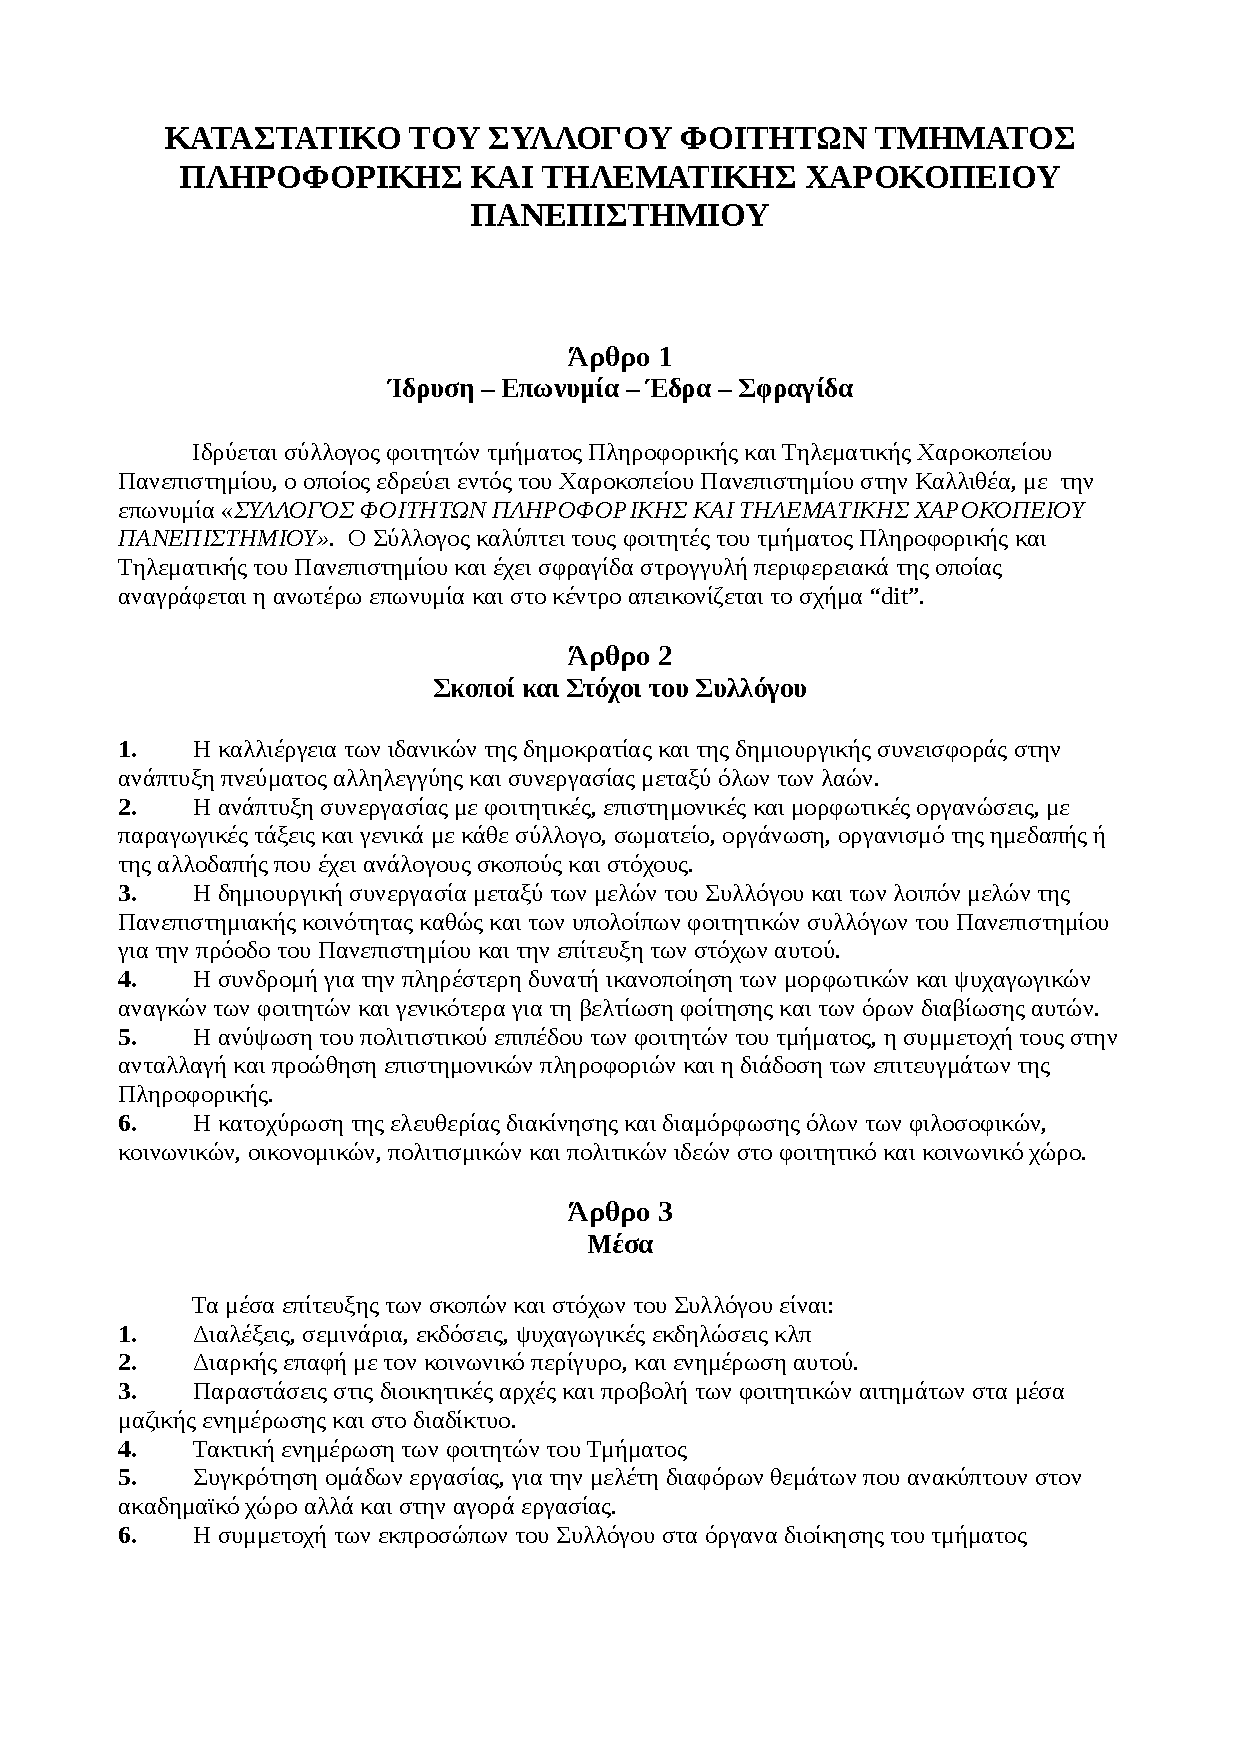
\includepdf[pages={1-8}]{katastatiko.pdf}
\end{document}
